\documentclass{sigkddExp}
\usepackage{graphicx, caption, subcaption}
%%%%%%%%%%%%%%%%%%%%%%%%%%%%%%%%%%%%%%%%%%%%%%%%%%%%%%%%%%
% TITLE
%%%%%%%%%%%%%%%%%%%%%%%%%%%%%%%%%%%%%%%%%%%%%%%%%%%%%%%%%%
%Title will probably change
\title{[PAPER DROP 2]\\
Predicting crime rates using taxi rides data}


%%%%%%%%%%%%%%%%%%%%%%%%%%%%%%%%%%%%%%%%%%%%%%%%%%%%%%%%%%
% AUTHORS
%%%%%%%%%%%%%%%%%%%%%%%%%%%%%%%%%%%%%%%%%%%%%%%%%%%%%%%%%%
\numberofauthors{3}
\author{
\alignauthor Carlos Petricioli \\
       % \affaddr{Computer Science Department}\\
       \affaddr{New York University}\\
       \affaddr{New York, USA}\\
       \email{petricioli@nyu.edu}
\alignauthor Valerie Angulo\\
       % \affaddr{Computer Science Department}\\
       \affaddr{New York University}\\
       \affaddr{New York, USA}\\
       \email{vaa238@nyu.edu}
\alignauthor Varsha Muralidharan \\
       % \affaddr{Computer Science Department}\\
       \affaddr{New York University}\\
       \affaddr{New York, USA}\\
       \email{vm1370@nyu.edu}
}


\begin{document}

\maketitle

%%%%%%%%%%%%%%%%%%%%%%%%%%%%%%%%%%%%%%%%%%%%%%%%%%%%%%%%%%
% ABSTRACT
%%%%%%%%%%%%%%%%%%%%%%%%%%%%%%%%%%%%%%%%%%%%%%%%%%%%%%%%%%
\begin{abstract}

Understanding and predicting crime is a crucial task in any major city. The objective of this study is to understand crime rates and its effects on how the use of taxis in New York City at a granular level. The idea  is that people react according to how secure they feel, which extends to their travel preferences. 
Our hypothesis is that people are less likely to walk in areas subjectively deemed more dangerous, and will instead opt to use more reliable and immediate transportation such as designated taxis. 
New York City will be used in this study as it provides a large amount of public data on crimes throughout the five boroughs along with an extensive amount of data from NYC yellow cab usage. 


\end{abstract}



%%%%%%%%%%%%%%%%%%%%%%%%%%%%%%%%%%%%%%%%%%%%%%%%%%%%%%%%%%
% INTRODUCTION
%%%%%%%%%%%%%%%%%%%%%%%%%%%%%%%%%%%%%%%%%%%%%%%%%%%%%%%%%%

\section{Motivation}

Understanding and predicting crime is a crucial task in any major city. 
The ability to understand criminal activity in a very delimited area adds depth to the current understanding of crime and  it provides a baseline to understand its effect on people's behavior. 
This question is relevant because it has a direct impact on the families economies since taking a taxi is the most expensive public transportation option and might also have an impact on people's health because there might be avoiding to walk to avoid crime which directly reduces peoples physical activity and might impact their health in the long run. 
This fact could translate into a much bigger public health issue for the city in the long run. %%% A LOT OF CITES NEEDED HERE.

%%Motivation in presentation slide
This analytic can help law enforcement predict areas of crime based on New Yorkers transportation habits. Those who live in an area are aware of the safety of their surroundings and this awareness can be represented by how comfortable residents may be in walking or taking the subway versus taking more immediate, more expensive, modes of transportation such as taxis. It is hypothesized that if someone feels unsafe in an area, they would be more likely to take a more direct and presumably safer mode of transportation such as a taxi. 

By analyzing the patterns of taxi usage in New York City, along with current crime data, law enforcement officials may be able to predict which areas will have a higher rate of crime in the future. This information can also be used as open source data, which would benefit the community and tourists by revealing taxi usage in regards to crime, and perhaps comforting people in using less expensive means of transportation and allowing them to save money in an expensive city.  
%%%


Specifically, we picked New York City because it has the largest  total number of offenses known to law enforcement by city crime according to the FBI's Uniform Crime Reporting \cite{fbiUniformCrime}, with a total of around 223 thousand for 2016 over cities like Los Angeles, Houston and Chicago, which have 156, 148 and
147 thousand offenses respectively. 
This provides the most vast crime dataset for this analysis.
Also, New York City has an Open Data Law which mandates that all public crime data be available online \cite{OpenDat}, which makes crime data collection easily accessible to the public.

\begin{figure}
\caption{Total number of reported crimes (2008 - 2017)}
\label{total_crimes}
\centering 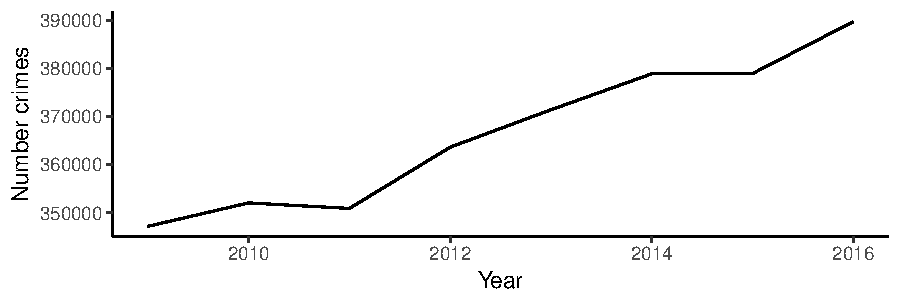
\includegraphics[width=.45\textwidth]{../img/total_crimes.pdf}
\end{figure}



% Our primary reason is thatThere are an abundance of transportation services available in New York City and taxi data is common enough to garner a big data set. 
%THIS IS NOT THEEEE PRIAMARY REASON ITS JUST CONVENIENT FOR US. THE PRIMARY REASON SHOULD BE THAT WE CONSIDER NYC INTERESTING FOR ITS BLAAA..., IT COULD BE ANYTHING BUT THERE ARE ABUNDANCE OF TRANSPORTANTION SERVICES IN MANY PLACES AND WE STILL PICKED NYC BECAUSE X.


% IN NOT SURE THIS IS ACUTALLY TRUE IF IT IS WE SHOULD CITE SOMETHING: 
       % It is also easy for individuals to choose a reliable taxi company, the NYC yellow taxi, which is a widely used and reputable taxi company. 
% With the abundance of transportation options, our study can explore transportation patterns such as taxi usage versus subway usage based on subway locations and taxi pickup/drop off coordinates. %ITS NOT VS SUBWAY USAGE BECASE WE CANNOT BE SURE OF THAT. IT SHOULD BE SOMETHING LIKE TAXI USAGE GIVEN THE PROXIMITY TO A SUBWAY STATION AT A GIVEN LOCATION.
\section{Introduction}

It is hard to argue that violence and crime is not a relevant factor that people take into consideration when commuting among the boroughs of New York city. 
So, this work assumes that that people want to minimize the time spent in locations they consider unsafe which  plays a roll in their transportation preferences affecting their taxi usage. 

What goes into an individuals subjective view of what is safe versus unsafe can be hard to gage. However, a lot can be inferred from an individuals behavior patterns.
One such pattern of behavior is transportation habits. The idea is to correlate taxi pickup and drop off information to the perceived level of crime activity in an area. 
It is inferred that people choose to not use public modes of transportation in areas where an individual feels unsafe or uncomfortable and will instead opt to use a more direct and safer source such as a designated taxi. 
% Through open source data of taxi trips, we hope to correlate peoples transportation behavior with the rate of crime activity in a given area. 



% Relating crime to transportation is important because it uses the knowledge of those who live in an area to predict which areas may be more prevalent to crime. %I DONT LIKE THIS SENTENCE HAHA. 
% This is an intuitive source of information that utilizes people and their knowledge of the city in crime prediction. %SAME HERE THIS IS A COMPLEX THING TO SAY WE SHOULD KEEP IT SIMPLE 

This study can give a look into what areas people avoid, allowing to geographically match the locations of crime activity to geographical pickup/drop off locations of taxi trips provided in the open source taxi data and can also provide information into the development of areas that become more or less crime ridden. 

To perform all the analysis, three main datasets were chosen.
The Taxi \& Limousine Commission (TLC) provide open data for all the rides in New York City since 2009 up to the present \cite{Taxi}. 
The crime data collected for this study contains historic \cite{NYPDHis} and current \cite{NYPDCur} records from NYPD complaint data, which has crimes reported since 2006 until present.
Data collected from the National Oceanic and Atmospheric Administration (NOAA) \cite{NOAA} is used as a third data source in order to provide a more controlled analysis. Specifically, hourly weather data  captured from three stations, Central Park, JFK airport, and La Guardia airport stations, is used as a possible explanation for taxi/crime patterns that do not correlate, seeing as weather is often a factor in the decision to take certain forms of transportation.

%NOT ACCURATE NOT HERE: For this study, we will compare the distance of taxi pickup locations to reported locations of crime activity. This is so that we can unite these two data sources based on geographic locations within the city. 

These three data sets were downloaded into a Hadoop cluster\footnote{NYU's High Perfomance Computing Hadoop cluster, Dumbo}, as shown in Figure \ref{figx}. Both crime and taxi data contain latitude and longitude data, which provide a very granular way of relating the datasets. 
This was achieved by a spatial join formulated as a Map/Reduce problem in order to exploit the benefits of the cluster. 
The problem was, how to join the  longitude and latitude coordinates for crime activity with the coordinates for taxi usage to a specific area  in New York City   in order to have a commonly defined location between the two sources.
Also, hourly weather data collected at three points, Central Park, LaGuardia and JFK, was assigned to each taxi ride by picking the data collected from the nearest station to the pickup location at a given time. 




%%%%%%%%%%%%%%%%%%%%%%%%%%%%%%%%%%%%%%%%%%%%%%%%%%%%%%%%%%
% RELATED WORK
%%%%%%%%%%%%%%%%%%%%%%%%%%%%%%%%%%%%%%%%%%%%%%%%%%%%%%%%%%

%%% THIS HAS TO BE MUCH MORE DETAILED
\section{Related Work}

There have been some studies on big data sources used in conjunction with crime data in order to understand and predict crime patterns. 
In one such study \cite{Wang16}, the authors propose to complement the traditional ways of predicting crime rates by including the use points of interest (POI) and taxi flow data in Chicago. 
In that study, it is hypothesized that taxi flows are ``hyper links'' within a city that connect locations, where they may be a proxy for broader patterns of population routine activity and mobility, commuting flows, and other forms of social and economic exchanges between two communities over space. The authors use POI to enhance the demographics information and use taxi flow as hyper links to enhance the geographical proximity correlation however, the temporal dimension of crime is not considered in depth. The problem in this study is population-centric, where the crime rate for Chicago is profiled in community areas that are well-defined and stable geographical regions. The proposed POI features and taxi links provide new perspectives in profiling the crime rate across community areas and the crime data collected in Chicago contains detailed information about the time, location and type of crime committed.

Other studies utilize crowd sourced data to predict crime patterns. In a recent study \cite{Bendler14}crowd sourcing of tweets was used as a virtual neighborhood watch in order to find crime patterns. The rough location for where the twitter post was sent can be determined by the social network provider or by geo-tags from the users phone. This study inferred that there was a correlation between an important event and the amount of tweets traced to a specific area, where an increase in the amount of tweets in a given area within a certain time span suggests an event was occurring at that time and place. The goal of this study was to predict and explain crimes in urban areas through tweet volume where crime and tweets were related through time and location. This study collected tweets and crime data in hourly blocks at Market Street in San Fransisco during a duration of three months. 

Urban crime has been correlated with different modes of communication data as well. The authors of a recent study \cite{Traunmueller14} presented a method to relate crime in London and people dynamics through the utilization of crime data records for the area of Greater London and data from a mobile telecommunication provider for details of people dynamics. Crime data was recorded with latitude/longitude coordinates whereas the telecommunication data was available as footfall in grids of varying sizes (smaller grids in central London as opposed to larger grids in less densely populated areas outside central London). While many people dynamics were looked at in depth in regards to crime, there were two major limitations in the study performed. One was that the crime data was recorded on a monthly basis whereas the telecommunications data recorded footfall on an hourly basis. This limitation is avoided in our study by grouping the data together by hour so that it is more cohesive. Because our study emphasizes time and location of taxi usage, crime activity and surrounding weather conditions, we have made sure that our three data sources share these conditions.

Various methods of mapping are explored in "The Utility of Hotspot Mapping for Predicting Spatial Patterns of Crime" \cite{Chainey}, which is of use to our study. Five different methods have been or are currently being utilized for crime mapping: point mapping, standard deviation spatial ellipses, thematic mapping of administrative units, grid thematic mapping and KDE (kernel density estimation). For this study, crime data was grouped by four types: burglary, street crime, vehicle theft and thefts from vehicles. Areas of high crime concentration (hotspots) in Central/North London were mapped using geocoded crime point data obtained from the Metropolitan Police covering the time period between January 2002 to December 2003. Two dates were chosen to be represented on the hotspot maps, one on Jan 1st as an unusual activity date and one on March 13th as a more ordinary activity date. The time data was sliced into 10 different time periods to avoid getting a map of a time range and perhaps having the map produce a strange result due to “unusual activity day” patterns. A Prediction Accuracy Index was used where the percentage of crime events for a specific time in a determined crime hotspot was divided by the percentage area of the hotspot compared to the total study area. The hotspot mapping techniques chosen for use in this study along with the methodologies being used were spatial ellipses (STAC: CrimeStat), thematic mapping of boundary areas (MapInfo), grid thematic mapping (MapInfo) and KDE (Hotspot Detective). After mapping the data, it was concluded that KDE is the best of the four methods for predicting spatial patterns of crime due to the accuracy in identifying the location, size, orientation and spatial distribution of the data. KDE uses point data along with two user defined parameters, search width and grid cell size. The street crime hotspot maps were best at predicting future street crime events compared to the other types of crime. This is because street crimes typically occur in areas where there are more shops, bars and other points of interest that give opportunity for street crimes to occur. 

%%%%%Carlos summary 2 has to be condensed%%%%
In the paper \cite{visCrime} the authors propose a spatial epidemiological analysis of crime to reveal uneven distributions of crime risks and spatial interaction between crime events. This article is intended to contribute to extending crime analyses from the spatial perspective to a spatiotemporal one, by proposing an exploratory method to comprehend space-time patterns of crime clusters using space-time statistics and 3D visualisation techniques. A number of studies have highlighted the importance of temporal aspects in crime concentrations is crucial for identifying appropriate crime reduction responses. For example, short-term or cyclic clusters would require a quick strategic action using policing resources, while stable clusters may require long-term efforts to modify social and built environments. However, less attention has been paid to the development of systematic analysis and representational methods of temporal dimensions, as compared to the geographic dimensions of crime epidemiology. Mapping crime at different time periods is probably the most common method to detect temporal changes in the distribution of crime clusters. In some cases, a research design may naturally lead to a pair of periods to be compared for testing a hypothesis on distributional changes of crime incidence. For example, in order to assess the impacts of social and built environmental changes caused by a large transportation project on the geographical distribution of crime, Ceccato and Haining (2004) used spatial scan statistics to assess the difference in geographic offence patterns over two periods of time, e.g. before and after the construction of a bridge across the Sweden- Denmark border. To evaluate the success of crime prevention measures frameworks of statistical testing to compare numbers of crimes in predefined regions before and after the measures were implemented. The dataset used in the study consists of occurrence points of snatch-and-run offences reported to the Kyoto Prefectural Police during the period 2003–2004. Snatch-and-run offences are a type of robbery committed on the street. In most situations, offenders snatch purses or bags and escape on a motorcycle. There has been an increase in such street crimes, thereby worsening the general perception of public safety in the society of Japan. To address this problem, police departments widely adopted GIS crime mapping. Kernel density estimation (KDE), devised for estimating a smooth empirical probability function (Silverman 1986), is now a commonly applied spatial analysis technique to transform a geographically distributed set of points into a density surface in a GIS environment. A crucial element of KDE is the selection of the bandwidth parameters. The bandwidths control the degree of smoothness in an estimated density surface. A large bandwidth leads to a smoother surface to emphasize statistically stable behaviour, though it may smooth out small but important spatio-temporal fluctuations from the true density distribution. By assuming that the expected number of crimes is geographically constant in the built-up area of the city, the authors apply the Poisson model of space-time scan statistics to a dataset consisting of crime event counts aggregated in each 500-m grid cell. The maximum radius of the cylindrical search window is set to 1 km based on a preliminary investigation of cluster sizes of the usual 2D crime mapping. Under the null assumption that cases of the event under study randomly occur following a Poisson distribution, Monte Carlo replications of the dataset enable the authors to obtain the simulated distribution of the likelihood ratio statistics l for significance testing of high density clusters. The authors generate 999 replications to obtain P-values, indicating the probability of the random appearance of an observed high crime density in a cylindrical window. The cluster defined by the cylindrical window with the lowest p-value is called the most likely cluster. Secondary clusters are also obtained for clusters that do not geographically overlap more likely clusters if their P-values are below the significance level. This visualisation methodology is designed to use descriptive and confirmative space-time statistics, which are the space-time kernel density estimation (STKDE) and space-time scan statistics (STSS), respectively. These two methodologies of space-time statistics used for 3D mapping are complementary. STSS rigidly specifies crime cluster domains that can be used for secondary analysis, such as evaluating temporal correlations of cases between detected cluster domains. However, the 3D method assumes that space-time domains of crime clusters are cylindrical. Three-dimensional mapping using STKDE draws fuzzy domains, indicating areas of high crime density but without clear boundaries. It can also be used to verify the assumption of STSS and to investigate more detailed space-time sequences of crime clusters. This is in contrast to the visualisation of STSS that statistically confirms anomalous concentrations of cases but might oversimplify the distribution of space-time concentrations.

%%%%%%%%%%%%% Varsha Summary 2 has to be condensed%%%%%%%%%%%%%%
In one study \cite{OUAC}, the authors proposed a method to predict crime in a geographic area using human behavioral data derived from a combination of mobile network activity and demographic information. Until the above method was presented, most existing research work had been from a people-centric perspective and made use of prior occurrences of crimes to identify patterns of crimes committed by the same offender/group of offenders, etc. A place- centric approach for crime hotspot detection and prediction as presented by the authors complements already existing methods and contributes to criminal studies and data-driven criminal studies. The datasets used are Criminal Cases Dataset (includes geo-location of all reported crimes with month and year tags, specific location of crime and type of crime (e.g. burglary, shoplifting, violent crime, etc.), Smartsteps Dataset (includes footfall per geographic division cell in London called Smartsteps cells and details about gender, age and home/work/ visitor group splits) and London Borough Profiles Dataset (contains 68 different metrics about the population of a geographical area (e.g. ethnicity, language, employment, etc.). The problem is treated as a classification task to predict if a particular cell will be a crime hotspot in the next month. Since the Smartsteps cell IDs, crime locations and borough profiles are not spatially linked, each crime event was mapped to a Smartsteps cell which it occurred closest to. The same was done for the borough profile dataset. The mean, median, standard deviation, min and max values and Shannon entropy is calculated for each Smartsteps variable. The criminal dataset was split into low crime (class 0) and high crime (class 1) classes depending on whether the number of crimes in a cell was higher than the median value. 80\% of data is used for training and 20\% for testing the classifier. Using Pearson correlation analysis, a large subset of the features are found to have strong mutual correlations. Hence, some of the features are dropped. The mean decrease in the Gini coefficient of inequality is used to rank features and to decide which features to select. From a set of over 6000 features, a subset of 68 features that are expected to have maximum influence in minimising error. Random Forest decision tree algorithm is found to have the best performance among other methods (regression, SVMs, neural networks). Accuracy, F1 and AUC score are the performance metrics used to evaluate the classification algorithm. It is seen that higher-level features extracted over a sequence of days have more predictive power than monthly extracted data. Features extracted from people who are ‘at home’ are found to be of high importance. The model is able to predict a crime hotpot in the following month with an accuracy of 70\%. This information can be used by the police departments to determine where to implement higher security.


\section{Design}

Figure \ref{figx} shows our data flow diagram\footnote{DUMBO refers to NYU's High Performance Computing Hadoop cluster}.  It shows that all three data sources were downloaded into a Hadoop cluster and cleaned in spark and later stored as Spark's SQL tables which can be read as Hive or Impala tables.

\begin{figure}
\caption{Data flow diagram}
\label{figx}
\centering 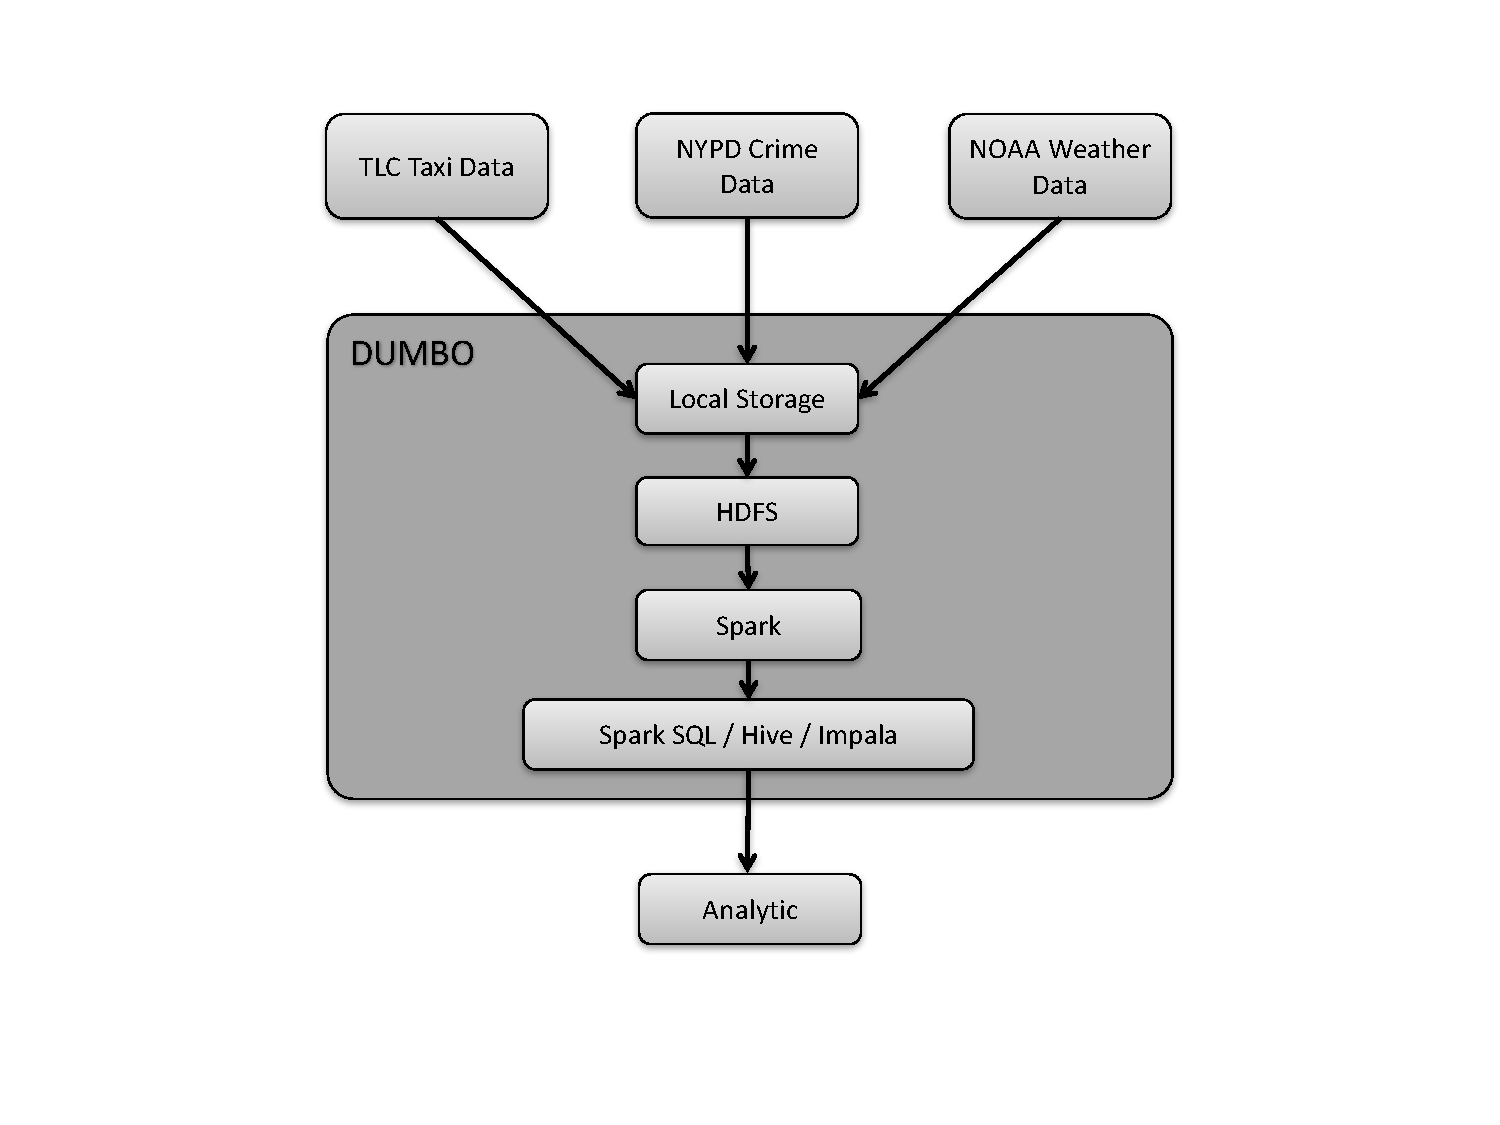
\includegraphics[width=.45\textwidth]{images/DesignFlowDiagram.pdf}
\end{figure}


\subsection{Getting and cleaning the data}

Getting the data was fairly easy because all three sets have APIs which provide a reliable and easy access.

\subsubsection{Crimes data}
There were a few anomalies that were found in the NYPD crime datasets. The two datasets (historic and current crime) at hand were for crimes that were reported from 2006 till present. However, certain records had incorrect or bad entries in the Crime Start and End Date-Time columns. For instance, there were several crimes reported to have occurred in the year 1016, which were assumed as a typological error for the year 2016. These records were fixed and used in the analytic. A few other records with year entries such as 1026 were dropped, as appropriate inferences could not be drawn. Certain records\footnote{Which make us wonder how much should we trust this dataset, but, still, it is what we have.} had timestamps of \texttt{24:00:00}, and were corrected to \texttt{00:00:00}.

\subsubsection{TLC data}
As expected there were complications while cleaning the Taxi rides data from TLC.

\subsection{Description of the data}


\subsection{Analytic}

Crime occurrences will be divided into  two levels: \textit{high crime} and  \textit{low crime} with respect to the total number of observed number crimes in a given period of time which will be defined later.
So crime level can be defined at every time $t$ an location $l$ as a binary variable for \textit{high crime} and \textit{low crime} when the total number of crime at is respectively higher and lower  than the average for that time and location.

To simplify things, any location is considered to have a  distance to a subway entrance equal to 0 if the location has any number available subway entrances,  1 if any of its neighbors location has a distance of 0 and 2 in every other case. \textbf{NOTE:} This assumption will be revised later to mark differences when a location has a lot vs just one entrance because it is important while making a very granular analysis.


Any taxi ride will be categorized as a \textit{short ride} if the distance form the pickup location to drop off location is considered as: could be walked in in less than a given time (i.e. 10 minutes) for an average person. And \textit{long ride} any other case.

With this implementation we  can to answer this type of questions:
\begin{enumerate}
       \item Is the average number of taxi pickups different in areas that have different levels of crime rates?

       \item Is the average number of taxi pickups different in areas that have different levels of crime rates grouping by the proximity of an area to a \textbf{subway}? 

       \item Is the average number of taxi pickups different in areas that have different levels of crime rates when we compare at times with and without \textbf{rain} (or different weather variables)?

       \item Does the average  number of \textbf{short} rides hve a different average number of taxi pickups  in areas that have different levels of crime rates  compared to the average of \textbf{long} rides?

       \item Does the answer of the previous questions change for special dates such as \textbf{holidays}?

       \item When categorized by the \textbf{severity of crime}, is the average number of taxi pickups different in areas that have different levels of crime rates for a given level of severity in crimes?

       \item \textbf{Run away vs feel attracted} to crime. When there are ``high profiled'' crime incidents in a given location does the average number of drop offs is greater, lower or similar to the average?\footnote{\textbf{NOTE:} This is a similar question to \cite{Bendler14}.}

       \item Given crime rates changes across time for a given area, is the average number of taxi pickups  changing too? If so, same direction? With a time lag?
       does it lasts long? Does severity has an impact?

       \item How does the error in the prediction of crime rates changes when modeling it with traditional demographics vs the taxi rides vs both as features?\footnote{
       \textbf{NOTE:} This is the main question of the paper from KDD 2016 \cite{Wang16}. }

\end{enumerate}


\begin{figure}
\label{fig:zones}
    \centering
    \begin{subfigure}[t]{0.25\textwidth}
        \centering
        \label{fig:zones_shape}
        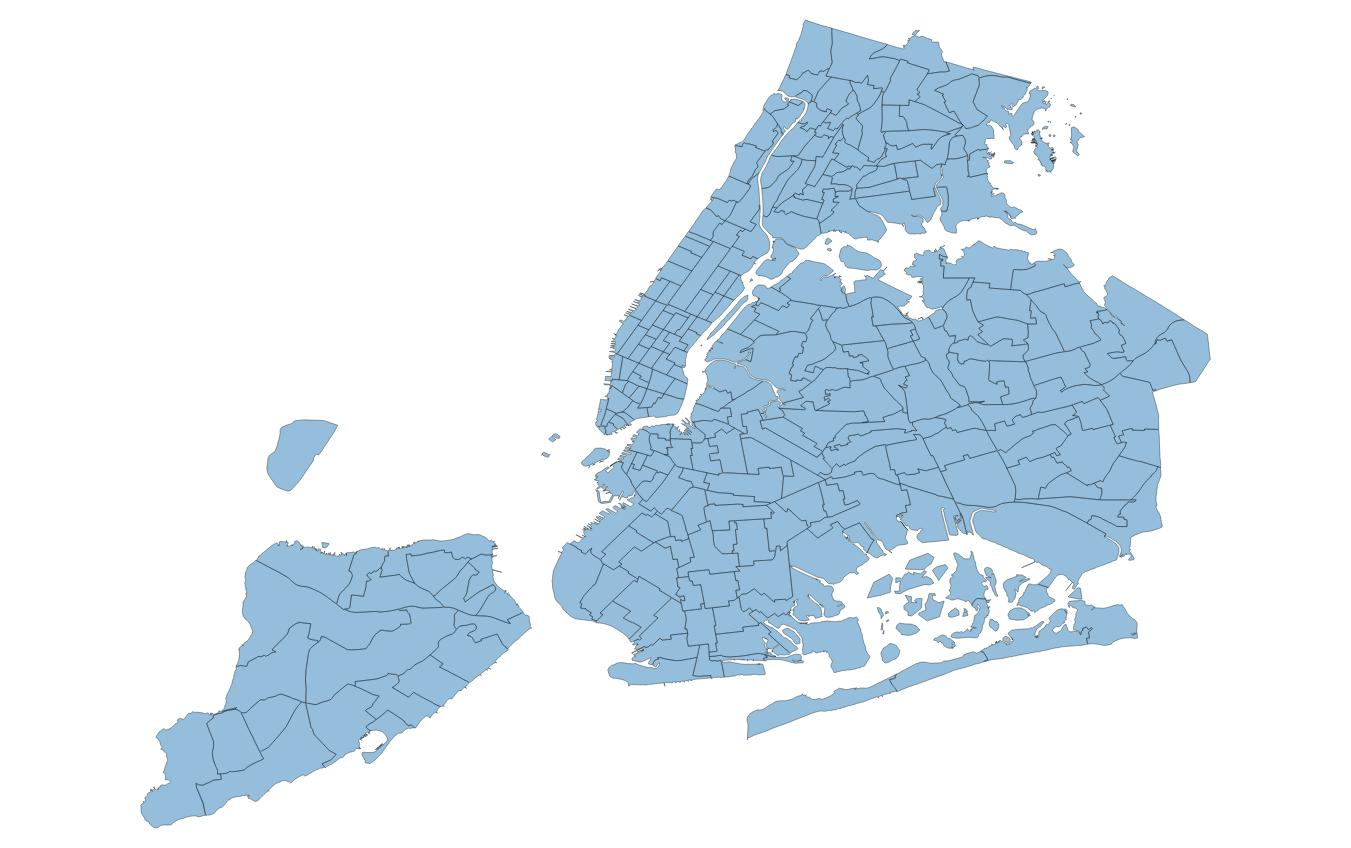
\includegraphics[height=1.2in]{images/taxi_zones_shape}
        \caption{Shape}
    \end{subfigure}%
    ~ 
    \begin{subfigure}[t]{0.25\textwidth}
        \centering
        \label{fig:zones_raster}
        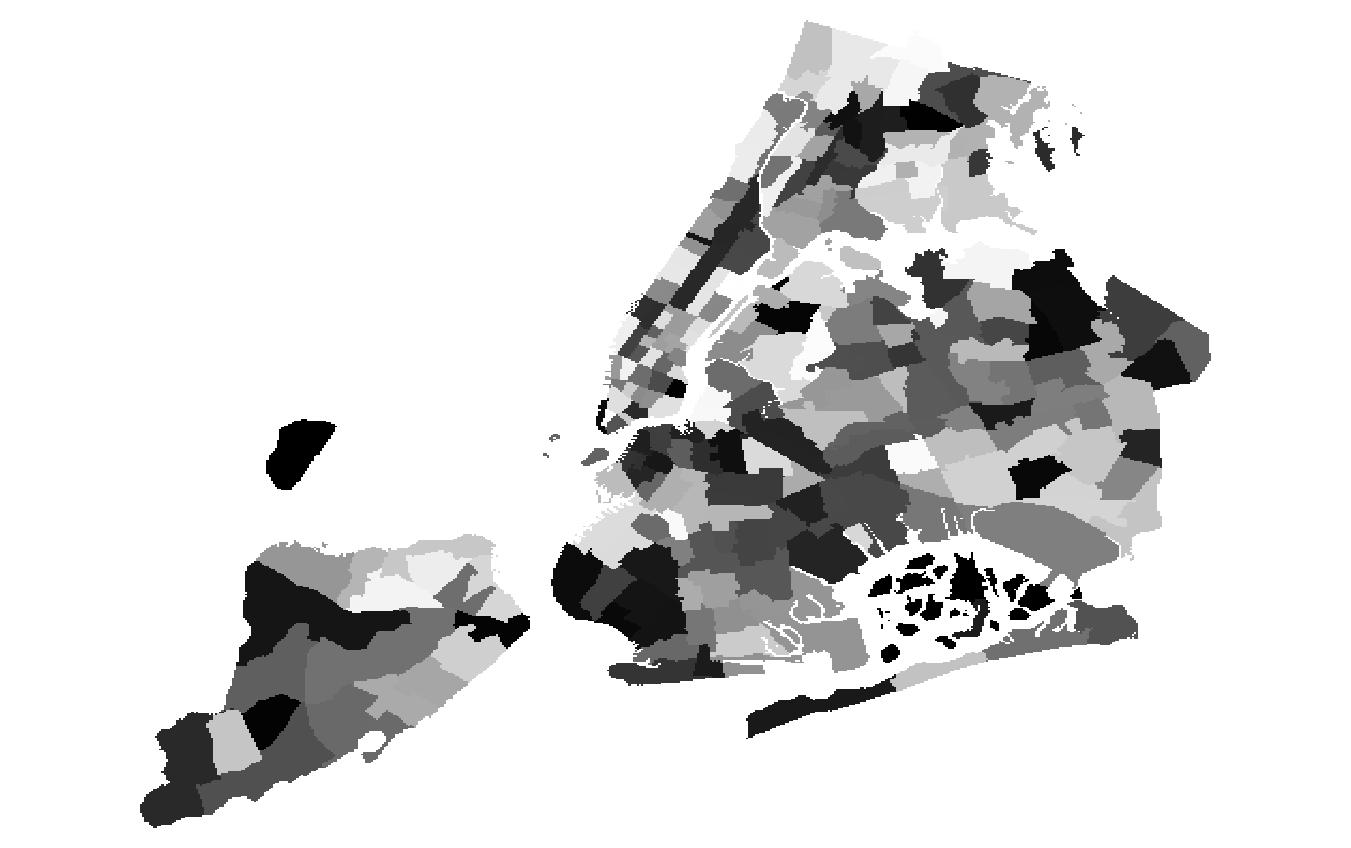
\includegraphics[height=1.2in]{images/taxi_zones_raster}
        \caption{Raster}
    \end{subfigure}
    ~ 
    \begin{subfigure}[t]{0.5\textwidth}
        \centering
        \label{fig:zones_both}
        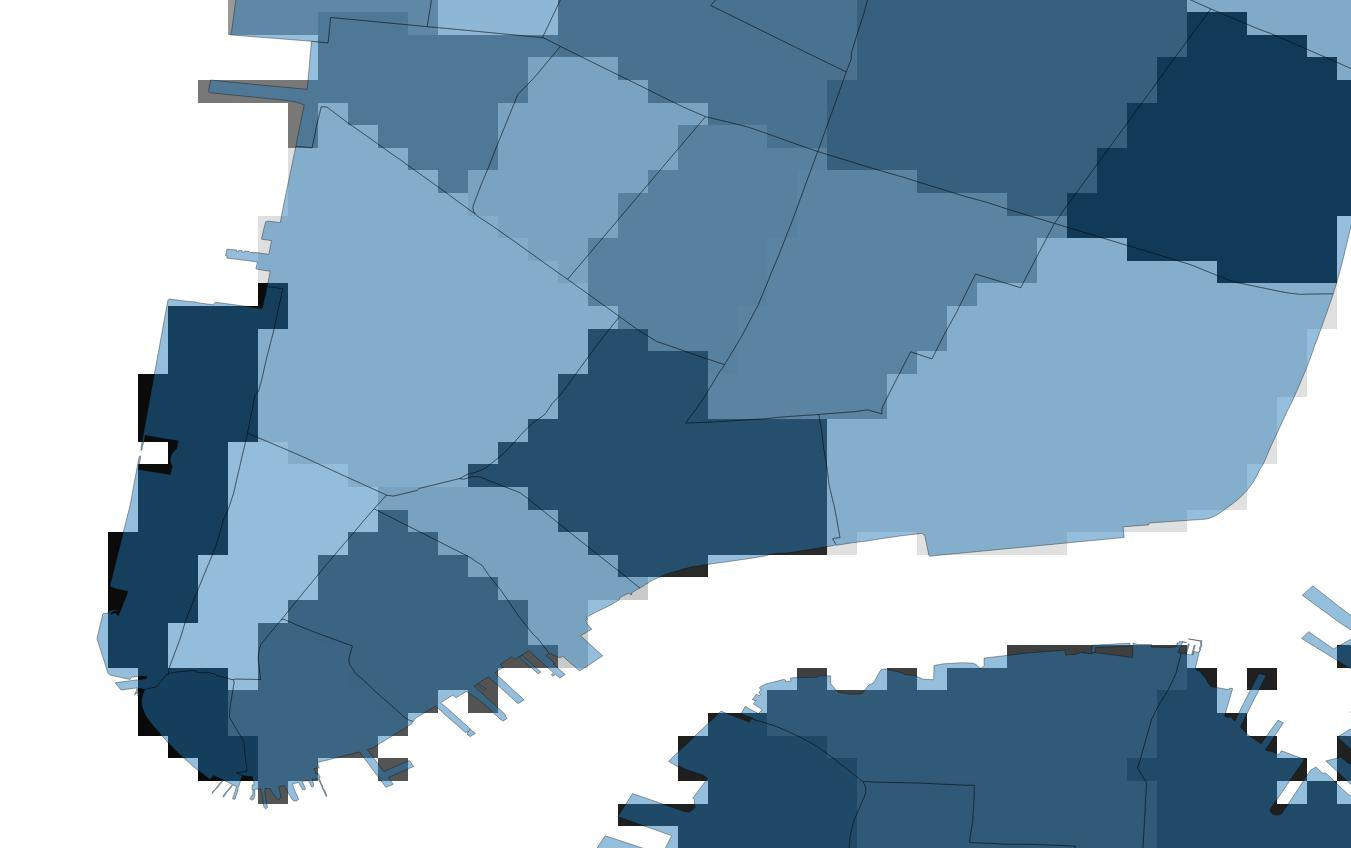
\includegraphics[width=0.5\textwidth]{images/both}
        \caption{Both}
    \end{subfigure}
    \caption{NYC Taxi zones file formats}
\end{figure}


\section{Limitations}
Our proposed method to quantitatively study crime rates in the city of New York intends to test the appropriateness of employing New York City TLC data and NOAA weather data as a suitable indicator for criminal activity in different New York City neighborhoods. Although the results of our study produce a considerable degree of validity, our work suffers from a few limitations. 
In the age of app-based transportation technology, companies such as Uber and Lyft are challenging the age-old taxi industry. 
A significant portion of the city's population makes use of these options over New York City taxis because of numerous reasons. 
For one, Uber's new strategy of making their services more available in the outer boroughs of New York City where taxis are scarce and access to public transport is not easy. Nevertheless, the TLC industry is still strong and serves roughly 50\% of city-wide taxi users.
%%%%%%%%%%%%%%%%%%%%%%%%%%%%%%%%%%%%%%%%%%%%% 
%%CITATION NEADED HEEERE for percentage of taxi usage
%%%%%%%%%%%%%%%%%%%%%%%%%%%%%%%%%%%%%%%%%%%


%%%%%%%%%%%%%%%%%%%%%%%%%%%%%%%%%%%%%%%%%%%%%%%%%%%%%%%%%%
% CONCLUSIONS
%%%%%%%%%%%%%%%%%%%%%%%%%%%%%%%%%%%%%%%%%%%%%%%%%%%%%%%%%%

% \section{Conclusions}
% This paragraph will end the body of this sample document.
% Remember that you might still have Acknowledgements or
% Appendices; brief samples of these
% follow.  There is still the Bibliography to deal with; and
% we will make a disclaimer about that here: with the exception
% of the reference to the \LaTeX\ book, the citations in
% this paper are to articles which have nothing to
% do with the present subject and are used as
% examples only.
%\end{document}  % This is where a 'short' article might terminate



%%%%%%%%%%%%%%%%%%%%%%%%%%%%%%%%%%%%%%%%%%%%%%%%%%%%%%%%%%
%ACKNOWLEDGEMENTS are optional
%%%%%%%%%%%%%%%%%%%%%%%%%%%%%%%%%%%%%%%%%%%%%%%%%%%%%%%%%%
% \section{Acknowledgments}
% This section is optional; it is a location for you
% to acknowledge grants, funding, editing assistance and
% what have you.  In the present case, for example, the
% authors would like to thank Gerald Murray of ACM for
% his help in codifying this \textit{Author's Guide}
% and the \textbf{.cls} and \textbf{.tex} files that it describes.



%%%%%%%%%%%%%%%%%%%%%%%%%%%%%%%%%%%%%%%%%%%%%%%%%%%%%%%%%%
% REFERENCES
%%%%%%%%%%%%%%%%%%%%%%%%%%%%%%%%%%%%%%%%%%%%%%%%%%%%%%%%%%
% ACM needs 'a single self-contained file'! SO WE'll NEED TO CHANGE THIS AT THE END.
\bibliographystyle{abbrv}
\bibliography{biblio} 



%%%%%%%%%%%%%%%%%%%%%%%%%%%%%%%%%%%%%%%%%%%%%%%%%%%%%%%%%%
% APPENDIX
%%%%%%%%%%%%%%%%%%%%%%%%%%%%%%%%%%%%%%%%%%%%%%%%%%%%%%%%%%
%APPENDICES are optional
% \balancecolumns
% \appendix
% %Appendix A
% \section{Headings in Appendices}


\end{document}
